%! TeX program = xelatex
\newcommand{\PFF}[1]{./body/aux/image-formation/#1}
\documentclass[../ml-ct.tex]{subfiles}
\begin{document}
\chapter{Image Formation}%
\label{chap:image-formation}
\myepigraph{Gradually he can see the reflections of people and things in water and then later see the people and things themselves.}{Plato}{Republic, VII, Allegory of the Cave}

\minitoc%
In the previous chapter we discussed the underlying physical principles as well as how these principles can concretely be used in implementing scanners.
Here, we want to investigate the mathematics of image acquisition and specifically reconstruction.
Recall that in \xray\ \gls{ct}, the fundamental measurement is a line integral of the linear attenuation coefficient \( \mu(x, E) \).
Specifically, assuming narrow beam geometry, we can relate the measured intensity \( I_d \) at the detector to the source spectrum \( S_0(E) \) with
\begin{equation}
	I_d = \int_0^{\Emax} S_0(\epsilon)\epsilon \exp{\left( -\int_0^d \mu(\chi, \epsilon)\ \dd \chi  \right)}\ \dd \epsilon.\label{eq:image:full line int}
\end{equation}

The above equation is in general intractable because of the energy dependence of the linear attenuation coefficient.
Therefore, the effective energy \( \Eeff \) is introduced, see~\cref{sssec:principles:polychromatic}, modifying~\cref{eq:image:full line int} to
\begin{equation}
	I_d = I_0 \exp{\left( -\int_0^d \mu(\chi, \Eeff)\ \dd \chi \right)}.
\end{equation}
Finally, we can rearrange this to yield the line integral of the linear attenuation
\begin{equation}
	g_d = -\log\left(\frac{I_d}{I_0}\right) = \int_0^d\mu(\chi,\Eeff)\ \dd \chi.
\end{equation}
In practice, the reference intensity \( I_0 \) can be measured for each detector in a calibration step.
\section{Forward Problem --- The Radon Transform}%
\label{sec:image:forward}
We have seen how a measurement in \gls{ct} corresponds to a line integral of \( \mu(x, \Eeff) \) along some path.
However,  what we desire is not the line integral, but the function \( \mu(x, \Eeff) \) itself for any point \( x \).
Thus, we have to ask the question whether it is possible to reconstruct \( \mu(x, \Eeff) \) given \enquote{all} its line integrals.
Fortunately, this question has been answered by Johann Radon approximately \num{50} years prior to the first practical experiments with the predecessors of modern \gls{ct}.

In \enquote{Über die Bestimmung von Funktionen durch ihre Integralwerte längs gewisser Mannigfaltigkeiten}~\cite{radon_bestimmung_1917}, Radon showed that a function \( \Func{f}{\R^2}{\R} \) is uniquely determined by its integrals along all lines.
Specifically, let
\begin{equation}
	\tcs = \begin{pmatrix} \cos\theta \\ \sin\theta \end{pmatrix}
\end{equation}
and 
\begin{equation}
	\tcsperp = \begin{pmatrix} -\sin\theta \\ \cos\theta \end{pmatrix}.
\end{equation}
Then, \( f \) is uniquely determined by
\begin{equation}
	\begin{aligned}
		\Func{F}{\R \times [0, \pi]&}{\R}, \\
		(r, \theta) & \mapsto \int_{-\infty}^{\infty} f(r\tcs + s\tcsperp)\ \dd s.
	\end{aligned}%
	\label{eq:image:radon trafo}
\end{equation}
This is true under mild assumptions about \( f \), which are in general fulfilled in \gls{ct}.
Specifically, we require
\begin{enumerate}
	\item \( f \) continuous,
	\item \(\displaystyle \int_{\R^2} \frac{|f(x)|}{\norm{x}_2}\ \dd x \) converges, and
	\item \(\displaystyle \lim_{r\rightarrow \infty} \int_{0}^{2\pi} f(x + r \tcs)\ \dd \theta = 0\ \forall x \in \R^2 \).
\end{enumerate}
Since the human body is finite in extent with finite \( \mu \) and the linear attenuation coefficient of air is \num{0}, the points are trivially fulfilled.
In what follows, we assume that the image of \( f \) is \( \R^+ \).

We call \( F \) the Radon transformed of \( f \), and refer to \( F(r, \theta^\prime ) \) as a \emph{projection} at a fixed angle \( \theta^\prime \).
To denote the transformation, we write \( F(r, \theta) = (\Radon f)(r, \theta) \).
Note that we may write~\cref{eq:image:radon trafo} as an integral over the two-dimensional Euclidean space as
\begin{equation}
	(\Radon f)(r, \theta) = \int_{\R^2} f(x) \indicator{\{\xi \in \R^2 \colon \xi^\top \tcs = r\}}{x}\ \dd x,%
	\label{eq:image:radon trafo euclid}
\end{equation}
where we used the masking property of the delta distribution
\begin{equation}
	\begin{aligned}
		\Func{\Indicator{\set{I}}}{\R^2&}{\{0, \infty\}}, \\
		x &\mapsto \begin{cases}
			\infty & \text{if}\ x \in \set{I}, \\
			0 & \text{else}.
		\end{cases}
	\end{aligned}
\end{equation}
We can draw \( F(r, \theta) \) in rectilinear coordinates to produce a \emph{sinogram}.
In scanner-geometry terms, we may think of \( r \) as the linear position of the detector, and we may think of \( \theta \) as the angle of rotation of the gantry with respect to the fixed patient-coordinate system.
To illustrate the ideas that were used above, we show an example in~\cref{fig:image:radon example}.
\begin{figure}
	\centering
	\begin{tikzpicture}
		\node at (0,0) {
			\begin{subfigure}{0.4\textwidth}
				\centering
				\includestandalone[height=4.5cm]{\PFF{geometry}}
				\caption{Geometry}%
				\label{fig:image:radon:geometry}
			\end{subfigure}\hfill%
			\begin{subfigure}{0.35\textwidth}
				\centering%
				\includestandalone[height=4.5cm]{\PFF{radon-example}}
				\caption{Example Projections}%
				\label{fig:image:radon:example}
			\end{subfigure}\hfill%
			\begin{subfigure}{0.2\textwidth}
				\centering
				\includestandalone[height=4.5cm]{\PFF{sinogram}}
				\caption{Sinogram}%
				\label{fig:image:radon:sinogram}
			\end{subfigure}
		};
		\begin{scope}[overlay]
			\draw[->] (2.8, 2) to [out=30,in=90] (5.85, 2.27);
			\draw[->] (1.2, -1.4) to [out=-70,in=-90] (5.1, -1.82);
		\end{scope}
	\end{tikzpicture}
	\caption[Visualization of the projection geometry in Computed Tomography.]{%
		In~\subref{fig:image:radon:geometry}, we show the interpretation of \( \tcs, \tcsperp, r, s\).
		Note that \( \{ x \in \R^2 \colon x^\top\tcs = r \} \) and \( \{ r\tcs + s\tcsperp \}, s \in \R \) describe the same line in the plane.
		In~\subref{fig:image:radon:example}, the projections \( F(r, \SI{130}{\degree}) \) and \( F(r, \SI{20}{\degree}) \) of some function \( f(x) \) are visualized, with the corresponding vertical lines in the sinogram~\subref{fig:image:radon:sinogram}.
		For visualization purposes, we only show \( \supp(f) \), and the color-bar is shown on the right.
	}%
	\label{fig:image:radon example}
\end{figure}

We want to note that, by construction, we are only considering integrals along parallel rays in each projection.
This is theoretically only fulfilled in first-generations scanners, which are no longer used in medical applications.
However, the following considerations can also be applied to fan beam geometries by adapting them accordingly.
As such, going through the principles of the simplest geometries is a useful exercise.
\section{The Inverse Problem}
In the previous section, we specified the forward model by fixing the geometry and introducing some notation.
Further, we hinted at the fact that Radon proved that any function can be uniquely reconstructed given its Radon transform.
In this section, we will discuss some concrete reconstruction algorithms.
Loosely speaking, the reconstruction algorithms can be divided into two categories: \enquote{analytic} and \enquote{algebraic}.
Analytic reconstruction essentially aims to reconstruct \( f \) from~\cref{eq:image:radon trafo} or~\cref{eq:image:radon trafo euclid}, while algebraic reconstruction techniques aim to solve the linear equation systems that arise in practice.
In other words, analytic reconstruction solves the continuous model, while algebraic reconstruction solves the fully discretized model.
We will point out correspondences between the two when they arise.
\subsection{Simple Back-Projection}%
\label{ssec:image:sbp}
Considering the forward operation described in~\cref{sec:image:forward}, one possible reconstruction method is tempting:
What happens when we conceptually \enquote{reverse} the acquisition process?
Specifically, consider a projection \( F(r, \theta^\prime) \) at some angle \( \theta^\prime \in [0,\pi] \).
As previously described, for a given \( r^\prime \in \R \), \( F(r^\prime, \theta^\prime) \) is given by the integral of the desired function \( f \) along the line \( x\tp\tcs^\prime = r^\prime \), where \( \tcs^\prime = {(\cos\theta^\prime, \sin\theta^\prime)}\tp \).
Intuitively, the reverse of this would be to smear \( F(r^\prime, \theta^\prime) \) along \( x\tp\tcs^\prime = r^\prime \), i.e.\ to \enquote{back-project} it.
If we do this for all \( r \) and \( \theta \), we get the \emph{back-projected} image.

Mathematically, let \( F = \Radon f \), then the back-projected image \( \Func{b}{\R^2}{\R} \) is
\begin{equation}
	b(x) = \int_0^\pi F(x\tp \tcs, \theta)\ \dd \theta.%
	\label{eq:image:simple backprojection}
\end{equation}
Notice that if \( \supp(f) \neq \emptyset \) it follows that \( b(x) > 0\ \forall x \).
It is immediately clear that this is a drawback if we consider some \( x^\prime \notin \supp(f) \).
We can conclude that \( b \) is in general not a faithful reconstruction of \( f \).
We illustrate \gls{sbp} for a toy example in~\cref{fig:image:simple backprojection example}.
\begin{figure}
	\centering
	\scalebox{0.47}{
	\begin{tikzpicture}
		\begin{scope}[scale=0.8]
			\node[scale=0.8, xscale=-1] at (0, -0.2) {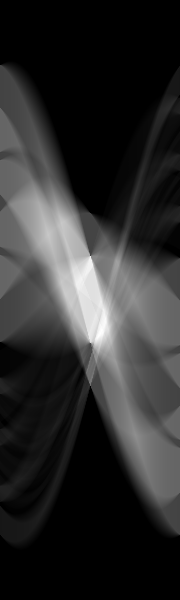
\includegraphics[height=9cm,width=4cm]{./figures/image-formation/sinogram.png}};
			\draw[-latex] (-2.2, 0) -- ++(4.5, 0) node [right] {\( \theta \)};
			\draw[-latex] (-2, -5) -- ++(0, 10) node [above] {\( r \)};
			\draw (2, 0.2) -- ++(0, -0.4) node [below] {\( \pi \)};
			\node at (-2, 0) [below left] {\( 0 \)};
			\coordinate (20deg low) at (-1.5555556, -4.7);
			\coordinate (130deg high) at (0.8888888, 4.3);
			\draw [red, loosely dashed] (20deg low) -- ++(0, 9);
			\draw [red, loosely dashed] (0.8888888, -4.7) -- (130deg high);
		\end{scope}
		\begin{scope}[shift={(7,0)}]
			\begin{scope}[shift={(-70:1cm)}]
				\begin{axis}[
					axis lines=middle, axis line style={-latex},
					anchor={(220,0)}, rotate around={20:(current axis.origin)},
					width=8.1cm, height=3.0cm,
					xlabel={\(r\)}, x label style={rotate=20,below=1mm},
					ylabel={\(F(r, \SI{20}{\degree})\)}, y label style={rotate=20,above=0mm},
					enlarge x limits=0.05,
					enlarge y limits=0.2,
					xtick=\empty,
					ytick=\empty,
				]
				\addplot[color=black,smooth] table[col sep=comma, header=false, x index=0, y index=1] {./figures/image-formation/radon.csv};
				\end{axis}
			\end{scope}
			\draw[gray, dashed] (-2.35, -0.45) -- ++(-70:4.7cm);
			\draw[gray, dashed] (2.35, -0.57) -- ++(-70:3cm);
			\node at (0, 0) {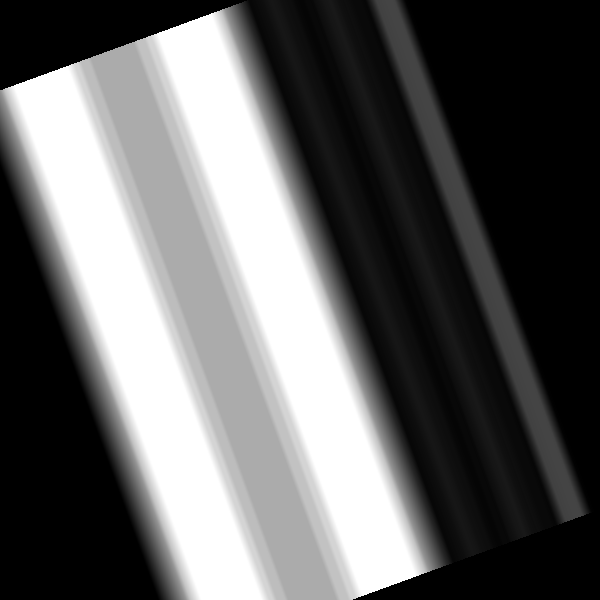
\includegraphics[trim=0cm 6cm 0cm 6cm, clip, width=6cm]{./figures/image-formation/bp20.png}};
			\draw[-latex] (0, 0) -- ++(4, 0) node [right] {\( x_1 \)};
			\draw[-latex] (0, 0) -- ++(0, 2) node [above] {\( x_2 \)};
			\draw[red] (2.21, -0.72) circle (0.3);
		\end{scope}
		\begin{scope}[shift={(16,0)}]
			\begin{scope}[shift={(40:-7cm)}]
				\begin{axis}[
					axis lines=middle, axis line style={-latex},
					anchor={(245,0)}, rotate around={-50:(current axis.origin)},
					width=8.15cm, height=3cm,
					xlabel={\(r\)}, x label style={rotate=-40,below=1mm},
					ylabel={\(F(r, \SI{130}{\degree})\)}, y label style={rotate=-50,above=0mm},
					enlarge x limits=0.05,
					xtick=\empty,
					ytick=\empty,
				]
					\addplot[color=black,smooth] table[col sep=comma, header=false, x index=0, y index=2] {./figures/image-formation/radon.csv};
				\end{axis}
			\end{scope}
			\draw[gray, dashed] (-2.35, 0.45) -- ++(40:5.9cm);
			\draw[gray, dashed] (2.35, -0.85) -- ++(40:4cm);
			\node at (0, 0) {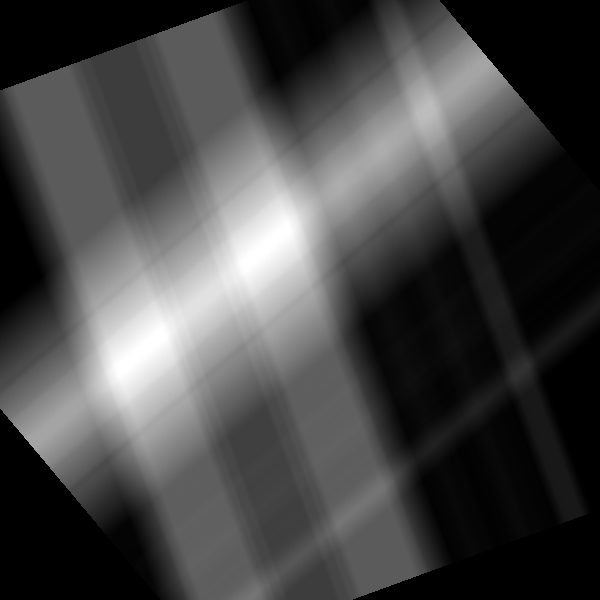
\includegraphics[trim=0cm 6cm 0cm 6cm, clip, width=6cm]{./figures/image-formation/bp130.png}};
			\draw[-latex] (0, 0) -- ++(4, 0) node [right] {\( x_1 \)};
			\draw[-latex] (0, 0) -- ++(0, 2) node [above] {\( x_2 \)};
			\draw[red] (2.21, -0.72) circle (0.3);
		\end{scope}
		\begin{scope}[shift={(25,0)}]
			\node at (0, 0) {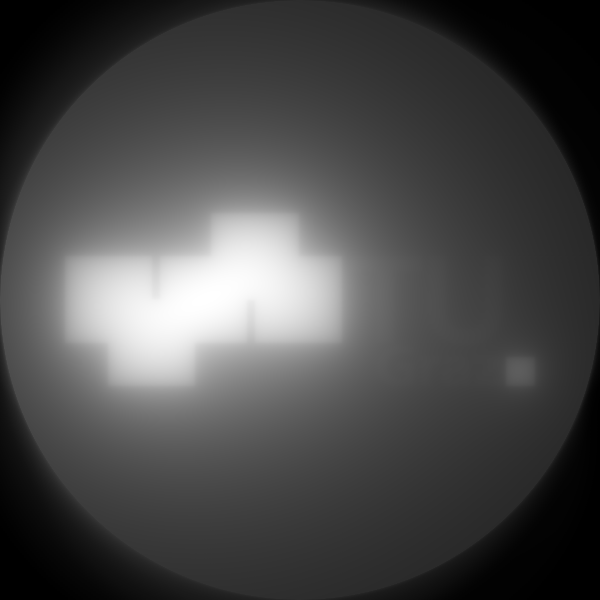
\includegraphics[trim=0cm 6cm 0cm 6cm, clip, width=6cm]{./figures/image-formation/bpfull.png}};
			\draw[red] (2.21, -0.72) circle (0.3);
			\draw[-latex] (0, 0) -- ++(4, 0) node [right] {\( x_1 \)};
			\draw[-latex] (0, 0) -- ++(0, 2) node [above] {\( x_2 \)};
		\end{scope}
		\begin{scope}[overlay]
			\draw [-latex] (20deg low) to[out=-60, in=200] ++(6.2, -0.9);
			\draw [-latex] (130deg high) to[out=60, in=130] ++(15.5, 1.3);
		\end{scope}
	\end{tikzpicture}}
	\caption[The Simple Back-Projection Algorithm.]{
		Illustration of the \gls{sbp} algorithm: For every angle \( \theta^\prime \) in the sinogram, we smear \( F(r, \theta^\prime) \) across the image.
		The red dot indicates the successive build-up of a distinct feature in the reconstruction process, and the reconstructed image is shown on the right.
	}%
	\label{fig:image:simple backprojection example}
\end{figure}

Let us examine the problem of \gls{sbp} in detail.
By substituting~\cref{eq:image:radon trafo euclid} into~\cref{eq:image:simple backprojection}, we find that
\begin{equation}
	b(x) = \int_0^\pi \int_{\R^2} f(\chi) \indicator{\{\xi \in \R^2 \colon \xi\tp \tcs = x\tp\tcs\}}{\chi}\ \dd \chi\ \dd \theta.
\end{equation}
We change the order of integration and note the equivalence \( \{\xi\in\R^2\colon\xi\tp\tcs = x\tp\tcs \} = \{ \xi\in\R^2 \colon {(\xi - x)}\tp\tcs = 0 \} \) to yield
\begin{equation}
	b(x) = \int_{\R^2} f(\chi) \left( \int_0^\pi \indicator{\{\xi\in\R^2\colon{(\xi - x )}\tp\tcs = 0\}}{\chi}\ \dd\theta \right)\ \dd \chi.
\end{equation}
Let \( \phi \) denote the angle between \( (\xi - x) \) and the \( x_1 \)-axis, then \( \{\xi\in\R^2\colon{(\xi - x )}\tp\tcs = 0\} = \{\xi\in\R^2\colon \norm{\xi - x}\cos(\phi - \theta) = 0\} \).
We now use
\begin{equation}
	\indicator{\{0\}}{g(x)} = \sum_{\{x_i\colon g(x_i) = 0\}} \left\vert\frac{\dd g}{\dd x}(x_i)\right\vert^{-1} \indicator{\{ x_i \}}{x},
\end{equation}
which is a well known identity in \(\delta\)-calculus~\cite{bracewell_fourier_1986}, and note that, assuming \( \xi \neq x \), \( \norm{\xi - x}\cos(\phi - \theta) = 0 \Leftrightarrow \phi - \theta = \pm\frac{\pi}{2} \).
We therefore obtain
\begin{equation}
	b(x) = \int_{\R^2} f(\chi) \left( \int_0^\pi \frac{\indicator{\{\pm\frac{\pi}{2}\}}{\theta}}{\norm{\chi - x}|\sin\pm\frac{\pi}{2}|}\ \dd \theta \right)\ \dd \chi.
\end{equation}
Since the delta distribution integrates to \num{1} and the denominator is independent of \( \theta \), this is easily simplified to
\begin{equation}
	b(x) = \int_{\R^2} f(\chi) \frac{1}{\norm{\chi - x}}\ \dd \chi.%
	\label{eq:image:backprojection as convolution}
\end{equation}

Clearly,~\cref{eq:image:backprojection as convolution} is a convolution.
Thus, one may equivalently write
\begin{equation}
	b(x) = f(x) * h(x),
\end{equation}
with the point spread function \( h(x) = \frac{1}{\norm{x}} \).
In general, this blurring makes \gls{sbp} useless, as too much diagnostic value is lost and more precise reconstruction algorithms with marginally higher computational cost exist.

However, one may ask the obvious question:
Since we know the blur function, what if we simply deconvolve \( b \) with \( h \), which can easily be done in the Fourier domain?
In fact, \( f \) can be faithfully reconstructed that way, and this is mathematically equivalent with one of the most popular reconstruction algorithms, namely \emph{\gls{fbp}} (although \gls{fbp} has practical benefits).
In what follows, we will introduce the famous \emph{Fourier Slice Theorem}, which gives rise to a family of Fourier-based reconstruction algorithms.
\subsection{Fourier Slice Theorem}
The Fourier Slice Theorem will allow us to derive an \enquote{inverse Radon transform}.
Consider the projection \( F(r, 0) \) of \( f \), i.e.
\begin{equation}
	F(r, 0) = \int_{-\infty}^{\infty} f(r, x_2)\ \dd x_2.%
	\label{eq:image:proj 0}
\end{equation}
The one-dimensional Fourier transform of \( F(r, 0) \) with respect to \( r \) is
\begin{equation}
	(\Fourier F)(\xi, 0) = \int_{-\infty}^\infty F(\chi, 0) \exp{(-\imagi2\pi\xi \chi)}\ \dd \chi
\end{equation}
with the imaginary unit \( \imagi \).
Substituting~\cref{eq:image:proj 0} yields
\begin{equation}
	\begin{aligned}
		(\Fourier F)(\xi, 0) & = \int_{-\infty}^{\infty} \int_{-\infty}^{\infty} f(x_1, x_2)\ \dd x_2  \exp{(-\imagi2\pi\xi x_1)}\ \dd x_1 \\
				  & = \int_{\R^2} f(x) \exp{(-\imagi2\pi(\xi x_1 + 0x_2))}\ \dd x = (\FFourier f)(\xi, 0)
	\end{aligned}
\end{equation}
In other words, the one-dimensional Fourier transform of the projection of \( f \) at \( \theta = 0 \) maps to the same values as the two-dimensional Fourier transform of \( f \) along the horizontal components.

If we consider \( F(r, 0) \) as the projection onto the \( x_1^\prime \) axis of some rotated coordinate system, the computation above holds.
In general, the two-dimensional Fourier transform of a function \( f \) rotated by some angle \( \alpha \) is also rotated by \( \alpha \) with respect to \( \FFourier f \).
Therefore, we proved the famous Fourier Slice Theorem, which we summarize as follows:
\begin{tcolorbox}[colback=lightgray]
	Let \( \Func{f}{\R^2}{\R} \), and let \( \FFourier f \) be its two-dimensional Fourier transform.
	Further, let \( F = \Radon f \) be its two-dimensional Radon transform, with \( \Fourier F \) its one-dimensional Fourier transform with respect to the affine parameter.
	Then, \( (\Fourier F)(\cdot, \theta) \) describes the values of \( \FFourier f \) on the radial line at angle \( \theta \).
	Thus, \begin{equation} (\Fourier F)(\rho, \theta) = (\FFourier f)(\rho \tcs).\label{eq:image:projection slice theorem} \end{equation}
\end{tcolorbox}
\subsection{Direct Fourier Inversion}
Knowing the Fourier Slice Theorem, another obvious reconstruction algorithm arises:
We can populate the \( \FFourier f \) along radial lines of angle \( \theta \) with \( (\Fourier F)(\rho, \theta) \), and then reconstruct \( f \) by
\begin{equation}
	f = \FFourier^{-1} (\FFourier f).
\end{equation}
This is schematically shown in~\cref{fig:image:direct fourier reconstruction}.
While straight forward in theory, this approach is usually not used in practice.
\begin{figure}
	\centering
	\includestandalone{\PFF{direct-fourier}}
	\caption[The Direct Fourier method for calculating the inverse Radon transform.]{%
		Schematic of the direct Fourier method for inverting the Radon transform.
		The error that arises during interpolation in the regridding step is what prevents this method from being used in practice.
	}%
	\label{fig:image:direct fourier reconstruction}
\end{figure}

In practice, scanners acquire a finite number of \( N \) projections \( \{ F(r, \theta_1), \dotsc, F(r, \theta_N) \} \) during one scanner rotation.
These measurements fill the Fourier space in radial lines, such that we need to interpolate the Cartesian grid prior to performing the inverse Fourier transform.
This process is called \emph{regridding} and is problematic in practice, since the distance between the radial streaks increases with the spatial frequency.
As such, the interpolation becomes less precise for higher frequencies, which encode the details in the image.
There exist schemes for non-uniform sampling in the Radon space to alleviate this issue, but they are not widely used and we do not discuss them here.
We refer the interested reader to~\cite{magnusson_linogram_1993} for further discussion.
\subsection{Filtered Back-Projection}
Fortunately, we can further modify the ideas of the direct Fourier inversion method to yield a reconstruction scheme that is very useful in practice.
We derive the basis equation of \gls{fbp} by considering the inverse Fourier transform of the image, i.e.
\begin{equation}
	f(x) = \int_{\R^2} (\FFourier f)(\xi) \exp{(\imagi 2\pi x\tp\xi)}\ \dd \xi.
\end{equation}
We introduce the polar coordinates \( \rho\tcs = \xi \), \( \dd \xi = \rho\ \dd \rho\ \dd \theta \), such that
\begin{equation}
	f(x) = \int_{0}^{2\pi} \int_{0}^{\infty} (\FFourier f)(\rho\tcs) \exp{(\imagi 2\pi \rho x\tp\tcs)}\ \rho\ \dd \rho\ \dd \theta,
\end{equation}
and note that we can equivalently scan the plane by (a very rigorous proof can be found in~\cite{buzug_computed_2008})
\begin{equation}
	f(x) = \int_{0}^{\pi} \int_{-\infty}^{\infty} (\FFourier f)(\rho\tcs) \exp{(\imagi 2\pi \rho x\tp\tcs)}\ |\rho|\ \dd \rho\ \dd \theta.
\end{equation}
With the Projection Slice Theorem~\cref{eq:image:projection slice theorem}, we may write
\begin{equation}
	f(x) = \int_{0}^{\pi} \int_{-\infty}^{\infty} |\rho| (\Fourier F)(\rho, \theta) \exp{(\imagi 2\pi \rho x\tp\tcs)}\ \dd \rho\ \dd \theta,
\end{equation}
or by noting that \( x\tp\tcs \) is nothing else than the \enquote{detector position} \( r \),
\begin{equation}
	f(x) = \int_{0}^{\pi} \underbrace{\left[\int_{-\infty}^{\infty} |\rho| (\Fourier F)(\rho, \theta) \exp{(\imagi 2\pi \rho r)}\ \dd \rho\right]}_{\tilde{F}(r, \theta)}\ \dd \theta.%
	\label{eq:image:filtered backprojection}
\end{equation}
\subsubsection{The Filtered Projections}
Let us now pay closer attention to the term in the square brackets, which we detail
\begin{equation}
	\tilde{F}(r, \theta) = \int_{-\infty}^{\infty} |\rho| (\Fourier F)(\rho, \theta) \exp{(\imagi 2\pi \rho r)}\ \dd \rho.
\end{equation}
This is exactly the one-dimensional inverse Fourier transform, weighted by \( |\rho| \).
In other words, if we disregard this factor, we would have \( \tilde{F} = \Fourier^{-1} \Fourier F = F \), which are the original projections.
By the famous convolution theorem, a multiplication in the Fourier domain corresponds to a convolution in the spatial domain.
Therefore, we may interpret \( |\rho| \) as a filter acting on the projections \( F \), i.e.\ \( \tilde{F} \) are filtered (read: convolved with some filter response) projections.

In the Fourier domain, the influence of \( |\rho| \) is relatively straight-forward:
Since the \enquote{radius} \( \rho \) essentially describes the frequency, we can immediately conclude that a multiplication with \( |\rho| \) in the Fourier domain is a high-pass filter.
On the other hand, since \( |\rho| \) is not square-integrable, we can not simply calculate its inverse Fourier transform to get the spatial filter.
However, we can detail the spatial filter by a limit process.
As an example, we may consider
\begin{equation}
	\Bigg(\Fourier \Bigg\{ \frac{\epsilon^2 - {(2\pi r)}^2}{{(\epsilon^2 + {(2\pi r)}^2)}^2} \Bigg\} \Bigg)(\rho) = |\rho| \exp{(-\epsilon |\rho|)},
\end{equation}
where \( \lim_{\epsilon \to 0} |\rho| \exp{(-\epsilon |\rho|)} = |\rho| \).
We show these functions in~\cref{fig:image:filters}.
\begin{figure}
	\centering
	\includestandalone[width=\textwidth]{\PFF{filters}}
	\caption[Spatial approximations for the linear ramp filter in the Fourier space.]{%
		Approximations for spatial convolution filters mimicking a multiplication with \( |\rho| \) in the Fourier domain.
	}%
	\label{fig:image:filters}
\end{figure}
In summary, in \gls{fbp}, we filter the projections by multiplying them with \( |\rho| \) in the frequency domain.
\subsubsection{The Back-Projection}
Let us now consider the outer integral in~\cref{eq:image:filtered backprojection}, namely
\begin{equation}
	f(x) = \int_0^\pi \tilde{F}(x\tp\tcs, \theta)\ \dd \theta.
\end{equation}
This is exactly~\cref{eq:image:simple backprojection}, where we replaced the projections \( F \) with their filtered counterparts \( \tilde{F} \).
The intuition is the same as discussed in~\cref{ssec:image:sbp}.
That is, in the image \( f(x) \) we smear \( \tilde{F}(r, \theta) \) along the line \( x\tp\tcs = r \).
Summing this over all \( \theta \in [0, \pi] \) (i.e.\ carrying out the integration) finally yields the reconstructed image \( f(x) \).

Thus, we summarize \gls{fbp} as a reconstruction algorithm in three steps:
\begin{tcolorbox}[colback=lightgray]
	Let \( F = \Radon f \) be the Radon transform of a function \( \Func{f}{\R^2}{R} \).
	Then, the \gls{fbp} algorithm for reconstructing \( f \) is as follows:
	\begin{enumerate}
		\item Calculate the one-dimensional Fourier transform \( (\Fourier F)(\rho, \theta) \) of \( F(r, \theta) \).
		\item High-pass filter \( (\Fourier F)(\rho, \theta) \) with \( |\rho| \) and compute the inverse Fourier transform \[ \tilde{F}(r, \theta) = \Fourier^{-1} \big\{|\rho| (\Fourier F)(\rho, \theta)\big\}. \]
		\item Back-project the filtered Radon transform \( \tilde{F} \) onto the image by \[ f(x) = \int_0^\pi \tilde{F}(x\tp\tcs, \theta)\ \dd \theta. \]
	\end{enumerate}
\end{tcolorbox}
We show reconstruction of our toy example in~\cref{fig:image:filtered backprojection example}, where we see that the image is faithfully reconstructed.
\begin{figure}
	\centering
	\scalebox{0.47}{
	\begin{tikzpicture}
		\begin{scope}[scale=0.8]
			\node[scale=0.8, xscale=-1] at (0, -0.2) {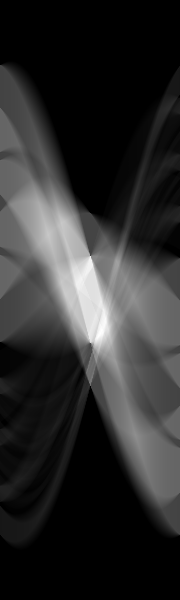
\includegraphics[height=9cm, width=4cm]{./figures/image-formation/sinogram.png}};
			\draw[-latex] (-2.2, 0) -- ++(4.5, 0) node [right] {\( \theta \)};
			\draw[-latex] (-2, -5) -- ++(0, 10) node [above] {\( r \)};
			\draw (2, 0.2) -- ++(0, -0.4) node [below] {\( \pi \)};
			\node at (-2, 0) [below left] {\( 0 \)};
			\coordinate (20deg low) at (-1.5555556, -4.7);
			\coordinate (130deg high) at (0.8888888, 4.3);
			\draw [red, loosely dashed] (20deg low) -- ++(0, 9);
			\draw [red, loosely dashed] (0.8888888, -4.7) -- (130deg high);
		\end{scope}
		\begin{scope}[shift={(7,0)}]
			\begin{scope}[shift={(-70:1cm)}]
				\begin{axis}[
					axis lines=middle, axis line style={-latex},
					anchor={(237,0)}, rotate around={20:(current axis.origin)},
					width=8.18cm, height=3.0cm,
					xlabel={\(r\)}, x label style={rotate=20,below=1mm},
					ylabel={\(\tilde{F}(r, \SI{20}{\degree})\)}, y label style={rotate=20,above=0mm},
					enlarge x limits=0.05,
					enlarge y limits=0.2,
					xtick=\empty,
					ytick=\empty,
				]
				\addplot[color=black,smooth] table[col sep=comma, header=false, x index=0, y index=1] {./figures/image-formation/radon_filtered.csv};
				\end{axis}
			\end{scope}
			\draw[gray, dashed] (-2.35, -0.45) -- ++(-70:4.7cm);
			\draw[gray, dashed] (2.35, -0.57) -- ++(-70:3cm);
			\node at (0, 0) {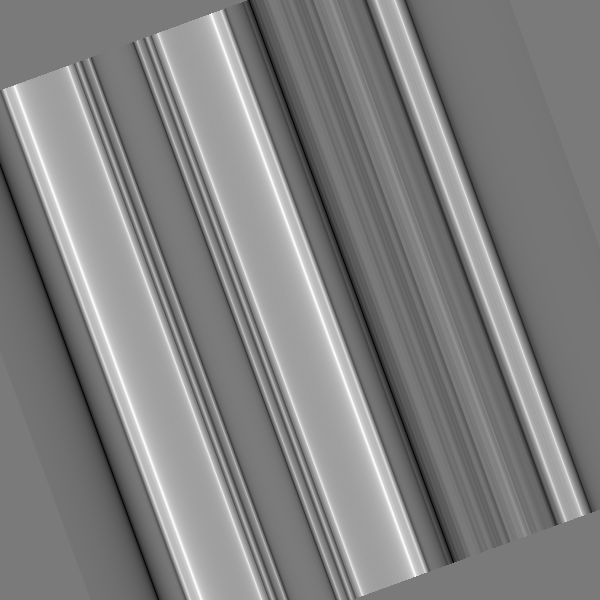
\includegraphics[trim=0cm 6cm 0cm 6cm, clip, width=6cm]{./figures/image-formation/fbp20.png}};
			\draw[-latex] (0, 0) -- ++(4, 0) node [right] {\( x_1 \)};
			\draw[-latex] (0, 0) -- ++(0, 2) node [above] {\( x_2 \)};
			\draw[red] (2.21, -0.72) circle (0.3);
		\end{scope}

		\begin{scope}[shift={(16,0)}]
			\begin{scope}[shift={(40:-7cm)}]
				\begin{axis}[
					axis lines=middle, axis line style={-latex},
					anchor={(185,0)}, rotate around={-50:(current axis.origin)},
					width=8.15cm, height=3cm,
					xlabel={\(r\)}, x label style={rotate=-40,below=1mm},
					ylabel={\(\tilde{F}(r, \SI{130}{\degree})\)}, y label style={rotate=-50,above=0mm},
					enlarge x limits=0.05,
					xtick=\empty,
					ytick=\empty,
				]
				\addplot[color=black,smooth] table[col sep=comma, header=false, x index=0, y index=2] {./figures/image-formation/radon_filtered.csv};
				\end{axis}
			\end{scope}
			\draw[gray, dashed] (-2.35, 0.45) -- ++(40:5.9cm);
			\draw[gray, dashed] (2.35, -0.85) -- ++(40:4cm);
			\node at (0, 0) {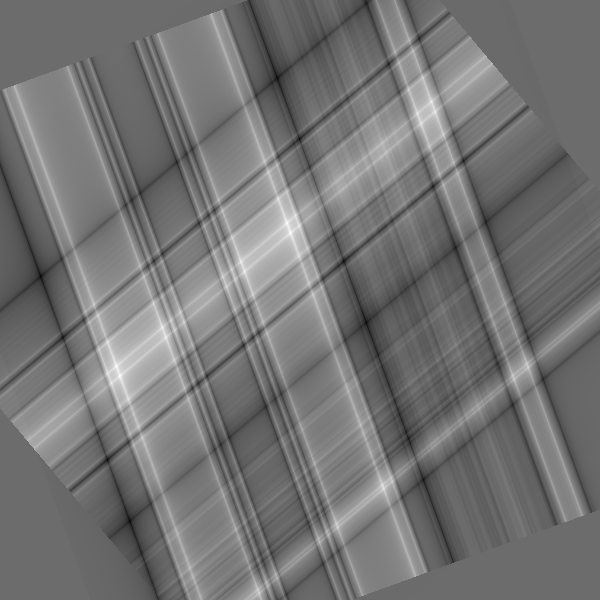
\includegraphics[trim=0cm 6cm 0cm 6cm, clip, width=6cm]{./figures/image-formation/fbp130.png}};
			\draw[-latex] (0, 0) -- ++(4, 0) node [right] {\( x_1 \)};
			\draw[-latex] (0, 0) -- ++(0, 2) node [above] {\( x_2 \)};
			\draw[red] (2.21, -0.72) circle (0.3);
		\end{scope}
		\begin{scope}[shift={(25,0)}]
			\node at (0, 0) {
\includegraphics[trim=0cm 6cm 0cm 6cm, clip, width=6cm]{./figures/image-formation/fbpfull.png}};
			\draw[red] (2.21, -0.72) circle (0.3);
			\draw[-latex] (0, 0) -- ++(4, 0) node [right] {\( x_1 \)};
			\draw[-latex] (0, 0) -- ++(0, 2) node [above] {\( x_2 \)};
		\end{scope}
		\begin{scope}[overlay]
			\node (f11) at (8, 7) {\( \mathcal{F}_1^{-1} \big\{|\rho| \mathcal{F}_1 \{\cdot\}\big\} \)};
			\node (f12) at (2, -5) {\( \mathcal{F}_1^{-1}\big\{ |\rho| \mathcal{F}_1 \{\cdot\}\big\}\)};
			\draw [-latex] (20deg low) to[out=-60, in=180] (f12) to[out=6, in=200] ++(2.8, 0.8);
			\draw [-latex] (130deg high) to[out=60, in=180] (f11) to[out=0, in=130] ++(8.8, -1.7);
		\end{scope}
	\end{tikzpicture}}
	\caption[The Filtered Back-Projection Algorithm.]{
		In the \gls{fbp} algorithm, the filtered projections \( \tilde{F}(r, \theta)\) are smeared across the image.
		The red circles indicate the successive build-up of a distinct feature in the image, and on the right we show the final reconstruction.
	}%
	\label{fig:image:filtered backprojection example}
\end{figure}

In the discussion about the \gls{sbp} algorithm, we hinted at the fact that one may also deconvolve the resulting image with the known blur function.
The corresponding reconstruction algorithm is sometimes referred to as \emph{filtered layergram}.
\gls{fbp} is mathematically equivalent to this, but it has a practical advantage:
Since the projections can be filtered independently, the reconstruction may start as soon as the first projection is acquired.
Moreover, looking at~\cref{fig:image:filters} we see that the spatial approximations of \( |\rho| \) have a small support.
Therefore, in practice it is often advantageous to completely circumvent all frequency domain calculations by implementing the spatial convolution rater than the Fourier domain multiplication.
The spatial kernel may also be calculated by windowing \( |\rho| \), or by simply choosing an appropriate kernel that may not be motivated by the frequency domain multiplication~\cite{ramachandran_reconstruction_1971}.
\section{Algebraic Reconstruction}
The reconstruction algorithms that were discussed in the previous sections are fast and derived in a rigorous framework.
While this may seem desired at first glance, it is actually a big weakness:
Due to wrong initial assumptions about the model, specifically that the \xray\ source is a monochromatic zero-width beam, these algorithms introduce typical artifacts in the reconstruction (see~\cref{sec:artifacts}).
Accounting for the energy dependence of the linear attenuation coefficient \( \mu \) is intractable mathematically and practically, and it is very hard to \enquote{inject} prior knowledge into the analytic reconstruction algorithms.

Algebraic (more specifically, iterative algebraic) methods allow for easy re-weighting of rays, and allow prior knowledge to be considered in the reconstruction.
This comes at the cost of much more computational expense, which is why typically analytic reconstruction dominated \gls{ct} historically.
However, the increase in computational power over the recent years has caused a gradual shift towards iterative methods.
In what follows, we want to detail the discretization of the model, and present typical algorithms for solving the arising linear system of equations.
We discuss linear inverse problems in the general sense, but put particular focus on the practical problems that arise specifically in \gls{ct} reconstruction.
\subsection{Discretized Model}
The analytic Fourier-based reconstruction algorithms are very principled in theory.
However, in practice the acquisition system is inherently discrete by design of the detector elements, and we store and view the reconstructed image on a discretized grid of picture elements.
Further, the integration along a line can not be realized practically, as the \xray\ beam will always have some \enquote{width} to it.

We represent the discretized image \( f \) as an \( N \)-dimensional vector, which corresponds to the \emph{flattened} image, i.e.\ is numbered in row-major order.
The projections \( p_i \) through \( f \) are easily modeled by introducing a weighting factor for each ray and pixel.
There exist many ways of defining the weighting, such as length of the ray in the pixel (assuming a zero-width ray) or the area of the intersection of the ray with the pixel.
In this case, for any pixel index \( j \), the weighting factor \( a_{ij} \) is, loosely speaking, the cross section of \( f_j \) with the \( i \)-th ray, divided by the total area of \( f_j \).
We show an example for the area integration framework schematically in~\cref{fig:image:discretized model}.
\begin{figure}
	\centering
	\includestandalone{\PFF{discretized-model}}
	\caption[Discretized model in Computed Tomography reconstruction.]{%
		The fully discretized model in \gls{ct} reconstruction, where the weights \( a_{ij} \) of the forward operator \( A \) are given by the area of the intersection of the \( i \)-th beam with the \( j \)-th pixel.
	}%
	\label{fig:image:discretized model}
\end{figure}
The evaluation of the forward operator is a very costly operation computationally, and much work has gone into efficiently computing it.
As an example, we refer the reader to~\cite{sungsoo_lookup_2017} for a look-up table-based area integration approach.

With~\cref{fig:image:discretized model}, we may now enumerate the equations as
\begin{equation}
	\begin{aligned}
		a_{11} f_1 + a_{12} f_2 + \cdots + a_{1N} f_N &= p_1 \\
		a_{21} f_1 + a_{22} f_2 + \cdots + a_{2N} f_N &= p_2 \\
							      & \vdots \\
		a_{M1} f_1 + a_{M2} f_2 + \cdots + a_{MN} f_N &= p_M,
	\end{aligned}
\end{equation}
or equivalently
\begin{equation}
	p = Af,%
	\label{eq:image:linear model}
\end{equation}
with the measurements \( p \in \R^M \), the design or system matrix \( A \in \R^{M\times N} \) and the image \( f \in \R^N \).
Throughout this work, we assume that \( A \) is known, and is appropriate for the problem.
We now note the equivalence with the continuous Radon transform by
\begin{equation}
	\begin{aligned}
		p &= Af \\
		&\Updownarrow \\
		F &= \Radon f_\text{cont},
	\end{aligned}
	\label{eq:image:matrix radon equivalence}
\end{equation}
i.e. \( p \) represents the sinogram in the Radon space and \( f \) holds the image values in the image domain.
The matrix \( A \) represents the linear map from the image space to the Radon space.

For example, assume we want to reconstruct an image \( f \in \R^N \) where \( N = \num{512} \times \num{512} = \num{262144} \).
Further, assume acquisition of \( M = \num{1000} \times \num{500} = \num{500000} \) rays, whereby \( N_D = \num{500} \) detectors acquire \( N_P = \num{1000} \) projection directions.
Then, the system matrix \( A \in \R^{\num{262144} \times \num{500000}} \) maps the image \( f \) to the sinogram \( p \).
We already see a practical problem arising:
Storing the system matrix \( A \) naively with \SI{32}{\bit} floating-point numbers would require approximately \SI{524}{\giga\byte} of storage.
Fortunately, as seen in~\cref{fig:image:discretized model}, the \( i \)-th ray does not intersect most pixels at all.
In other words, most entries \( a_{ij} \) in \( A \) are \num{0}, so we call \( A \) \enquote{sparse} and can store it efficiently.

The size and structure of \( A \) is still a problem.
Specifically, it is large without \enquote{simple} structure (to allow special inversion algorithms), such that in general we need \emph{iterative methods} to solve~\cref{eq:image:linear model}.
However, this allows to easily deal with irregularities in the measurement data, or to incorporate prior knowledge into the reconstruction problem.
We summarize the advantages and disadvantages of algebraic reconstruction over analytic reconstruction in~\cref{tab:image:analytic vs algebraic comparison}.
\begin{table}
	\centering
	\caption{Comparison of analytic reconstruction and algebraic reconstruction.}%
	\label{tab:image:analytic vs algebraic comparison}
	\begin{tabular}{cccc}
		Reconstruction & Model & Speed & Flexibility \\\toprule
		Analytic & continuous & fast & None\\
		Algebraic & discrete & slower & High \\\bottomrule
	\end{tabular}
\end{table}
\subsection{Solving the Linear System}
Let us consider~\cref{eq:image:linear model} in more detail.
In practice, the system will be overdetermined, since more projections than pixels are acquired.
Further, the measurements are noisy --- that is, in reality we only have access to noisy projection data \( p = Af + \nu \).
A well known solution to overdetermined, noisy systems is the least-squares solution
\begin{equation}
	\optimal{f}{LS} = \argmin_f \norm{Af - p}^2_2,
\end{equation}
which can be easily solved in closed form (disregarding the practical problem of actually \emph{calculating} it) as
\begin{equation}
	\optimal{f}{LS} = {(A\tp A)}^{-1} A\tp p = \pinv{A} p.
\end{equation}
Here, \( \pinv{A} = {(A\tp A)}^{-1} A\tp \) is the \emph{Moore-Penrose pseudo inverse} of \( A \).

In~\cref{eq:image:matrix radon equivalence}, we noted how \( A \) may be the discretized Radon transform, mapping from image space into Radon space.
The \emph{adjoint} operation, i.e.\ mapping from Radon space to image space is given by \( A\tp \).
Thus, we may interpret \( b = A\tp p \) as the \enquote{simple back-projection}.
Then it is clear that \( {(A\tp A)}^{-1} \) \enquote{filters} the back-projected image.
In this sense, \( \optimal{f}{LS} = {(A\tp A)}^{-1} A\tp p = {(A\tp A)}^{-1} b \) may be interpreted as the filtered layergram algorithm.
In the continuous discussion, we mentioned that the order of filtering and back-projection may be reversed.
Similarly, in the discrete setting we may write
\begin{equation}
	\optimal{f}{LS} = A\tp {(AA\tp)}^{-1} p,
\end{equation}
where \( {(AA\tp)}^{-1} \) is the linear frequency ramp filter, and \( A\tp \) is the back-projection operator.

Although we got valuable insight into the relationship between the continuous and discrete equations, the direct inversion does not work in practice because of the size of the matrices that need to be inverted.
In general,~\cref{eq:image:linear model} is solved by iterative methods, which we will discuss in the following section.
\subsection{Iterative Reconstruction}
Iterative reconstruction techniques aim to solve linear problems of the form~\cref{eq:image:linear model} without explicitly calculating the (generalized) inverse of \( A \).
The principle of all iterative reconstruction techniques can be summarized as follows:
\begin{enumerate}
	\item Forward Projection: Given the current estimate \( \optimal{f}{} \), compute the \enquote{expected} projections \( \hat{p} \).
	\item Correction: Compute the \enquote{error} \( (\hat{p} - p) \) between the expected projections and the measured projections, and properly normalize it.
	\item Back-Projection: Distribute the error back across all the pixels \( f_i^* \) that contributed to the difference.
\end{enumerate}
The iterative algorithms that are typically used in \gls{ct} reconstruction differ in the selection of pixels or beams that are considered simultaneously.
For instance, the forward projection may consider all pixels simultaneously or one pixel after the other, or we may operate on a ray-by-ray basis and correct only the pixels that contribute to the projection of the current ray.
\subsubsection{Kaczmarz Method}
Maybe the conceptually simplest algebraic reconstruction algorithm is the Kaczmarz method or method of projections~\cite{kaczmarz_angenaeherte_1937}, sometimes also (ambiguously) referred to simply as \gls{art}.
It is of the ray-based family of reconstruction techniques, where the corrections are applied on a ray-by-ray basis.
Specifically, the Kaczmarz iterations proceed by orthogonally projecting the images onto the hyperplanes defined by the projections of the individual rays, one after another.

Mathematically, this reads
\begin{equation}
	f \leftarrow f - \frac{A_i f - p_i}{\norm{A_i}_2^2} A_i\tp,\quad \forall i = 1,\dotsc,M,%
	\label{eq:image:kaczmarz}
\end{equation}
where \( A_i = ( a_{i1}, a_{i2}, \dotsc, a_{iN}) \) is the \( i \)-th row of \( A \).
Note how in~\cref{eq:image:kaczmarz} \( A_i f \) \enquote{forward projects} the image \( f \), the result of which is then compared to the measured projection \( p \).
The resulting error is normalized by \( \norm{A_i}_2^2 \), and subsequently \enquote{back projected} by \( A_i\tp \).
In this sense,~\cref{eq:image:kaczmarz} describes a cyclic gradient descent with adaptive step size \( \frac{1}{\norm{A_i}_2^2} \).

Typically we say that one iteration of the Kaczmarz algorithm is finished after all rows \( A_i, i = 1, \dotsc, M \) have been considered once.
Note that, since the systems arising in practical \gls{ct} are usually strongly overdetermined (i.e.\ \( M \gg N \)), most often the algorithm gives satisfactory results in one iteration.
In fact, practically the idea of an iteration is discarded and the \enquote{row index} \( i \) in~\cref{eq:image:kaczmarz} is often randomized.
We show the \gls{art} algorithm graphically in~\cref{fig:image:kaczmarz}.
\begin{figure}
	\centering
	\begin{subfigure}{0.39\textwidth}
		\centering
		\includestandalone[width=0.85\textwidth]{\PFF{kaczmarz}}
		\caption{}%
		\label{fig:image:kaczmarz toy}
	\end{subfigure}\hfill%
	\begin{subfigure}{0.6\textwidth}
		\centering
		\begin{tikzpicture}[scale=0.95]
			\foreach \i in {0, 1, ..., 8}
			{
				\pgfmathsetmacro\xx{floor(\i / 3) * -1.4};
				\pgfmathsetmacro\yy{Mod(\i, 3) * 3.1};
				\node at (\yy, \xx) {\includegraphics[trim=0cm 2.5cm 0cm 2.5cm, clip, width=2.8cm]{./figures/image-formation/kaczmarz/kaczmarz_\i.png}};
			}
		\end{tikzpicture}
		\caption{}%
		\label{fig:image:kaczmarz actual}
	\end{subfigure}\hfill%
	\caption[The Kaczmarz method to solving a linear system.]{%
		In~\subref{fig:image:kaczmarz toy}, we show the Kaczmarz iterations to solve a simple linear system, where the solution converges to \( \optimal{f}{} = {(3.5, 3.75)}\tp \).
		Each iteration is an orthogonal projection onto the hyperplane corresponding to one row in the system.
		In~\subref{fig:image:kaczmarz actual}, a tomographic reconstruction is shown, where after one iteration (lower right) the image is satisfactorily reconstructed.
	}%
	\label{fig:image:kaczmarz}
\end{figure}
\subsubsection{Simultaneous Iterative Reconstruction Technique}
An obvious modification to the \gls{art} algorithm is to consider not one, but all rays \emph{simultaneously} during one iteration.
The \gls{sirt} algorithm does just that:
Instead of updating the image successively to minimize the difference to each individual projection, it accumulates (and properly normalizes) the updates of \emph{all} rays during one iteration.
This modifies~\cref{eq:image:kaczmarz} to
\begin{equation}
	f \leftarrow f - C A\tp R (A f - p)%
	\label{eq:image:sirt}
\end{equation}
where \( C, R \) are diagonal matrices containing the inverse of the column- and row sums of \( A \), that is \( c_{jj} = {(\sum_i a_{ij})}^{-1} \) and \( r_{ii} = {(\sum_j a_{ij})}^{-1} \).
We show the iterations of the \gls{sirt} for the same problem as in~\cref{fig:image:kaczmarz} in~\cref{fig:image:sirt}.
\begin{figure}
	\centering
	\begin{subfigure}{0.39\textwidth}
		\centering
		\includestandalone[width=0.85\textwidth]{\PFF{sirt}}
		\caption{}%
		\label{fig:image:sirt toy}
	\end{subfigure}\hfill%
	\begin{subfigure}{0.6\textwidth}
		\centering
		\begin{tikzpicture}[scale=0.95]
			\pgfmathsetmacro\xx{floor(8 / 3) * -1.4};
			\pgfmathsetmacro\yy{Mod(8, 3) * 3.1};
			\node [fill=red!50!black] at (\yy, \xx) {
\includegraphics[trim=0cm 2.5cm 0cm 2.5cm, clip, width=2.8cm]{./figures/image-formation/sirt/sirt_100.png}};
			\foreach \i in {0, 1, ..., 7}
			{
				\pgfmathsetmacro\xx{floor(\i / 3) * -1.4};
				\pgfmathsetmacro\yy{Mod(\i, 3) * 3.1};
			\node at (\yy, \xx) {\includegraphics[trim=0cm 2.5cm 0cm 2.5cm, clip, width=2.8cm]{./figures/image-formation/sirt/sirt_\i.png}};
			}
		\end{tikzpicture}
		\caption{}%
		\label{fig:image:sirt actual}
	\end{subfigure}\hfill%
	\caption[The Simultaneous Iterative Reconstruction Technique for solving a linear system.]{%
		For the toy example in~\subref{fig:image:sirt toy}, after two \gls{sirt} iterations we converge to \( \optimal{f}{} \).
		In~\subref{fig:image:sirt toy}, we show the first \num{8} \gls{sirt} iterations (\( f^0 = 0 \)), and the final reconstruction after \num{100} iterations (highlighted in red).
	}%
	\label{fig:image:sirt}
\end{figure}
\subsubsection{Simultaneous Algebraic Reconstruction Technique}
Given \gls{art} and \gls{sirt}, it is natural to consider some \enquote{in-between} cases.
In \gls{sart}, one considers all rays of a particular projection simultaneously.
We may write this as
\begin{equation}
	f \leftarrow f - C_V A_V\tp R (A_V f - p),
\end{equation}
where \( A_V \in \R^{v \times N} \) contains the rows of \( A \) that correspond to a certain \enquote{view} (i.e.\ rotation angle), and \( C_V \) is contains the inverse of the corresponding column sums.

Of course, the field of linear systems is well studied and a plethora of algorithms exist for solving~\cref{eq:image:linear model}.
Other algorithms that are frequently used in \gls{ct} are the \gls{bicav}~\cite{censor_bicav_2001}, \gls{ossqs}~\cite{kamphuis_accelerated_1998,donghwan_accelerated_2011}, and \gls{cg}~\cite{fessler_conjugate_1999,ramani_splitting_2012}.
\section{Artifacts}%
\label{sec:artifacts}
In this section we will discuss typical artifacts in \gls{ct} imaging.
In the following discussion, we will take a broad definition of \enquote{artifact}.
Specifically, we define an artifact as any difference between the reconstruction and the measured function.
Artifacts may therefore appear because of the simplifications of the physical model, the fact that we only sample the radon transform, noise in the measurements, and movement of the patient during acquisition.
\subsection{Finite Beam Width}
In the derivation of the analytic reconstruction algorithms, it was always assumed that we can can integrate \( f \) along lines of no width.
Obviously, with real source-detector pairs this is not the case.
Even if we assume continuous sampling along the affine parameter \( r \), we would acquire the \emph{strip integral}
\begin{equation}
	(\Radon^w f)(r, \theta) = \int_{-\infty}^{\infty} w(u) (\Radon f)(r - u, \theta)\ \dd u,
\end{equation}
where \( \Func{w}{\R}{\R^+} \) is a weight function, sometimes called \emph{beam profile}.
It summarizes the effects of the finite-width source beam and detector pair.
\subsubsection{Image Convolution}
Shepp and Logan showed that the weighted Radon transform \( (\Radon^w f) \) is the Radon transform of a convolved signal \( f * k \)~\cite{shepp_fourier_1974}.
Specifically, \( \Radon^w f = \Radon (f * k) \) where \( \Func{k}{\R^2}{\R^+} \) is the radial function
\begin{equation}
	k(x) = -\frac{1}{\pi\norm{x}} \partial_{\norm{x}} \int_{\norm{x}}^\infty \frac{w(u)u}{\sqrt{u^2 - \norm{x}^2}}\ \dd u.
\end{equation}
Note that, if \( w \) has bounded support (which is a reasonable assumption in practice), then \( k \) also has finite support.
The following is an example pair \( (w, k) \):
\begin{equation}
	w(u) = \begin{cases}
		\frac{1}{2d} & \text{if}\ -d \leq u \leq d, \\
		0 & \text{else},
	\end{cases}\quad
	k(x) = \begin{cases}
		\frac{1}{2\pi d}\frac{1}{\sqrt{d^2 - \norm{x}^2}} & \text{if}\ 0 \leq \norm{x} \leq d, \\
		0 & \text{else}.
	\end{cases}
\end{equation}
We conclude that, even if we assume continuous sampling of \( (\Radon^w f)(r, \theta) \) along both \( (r, \theta) \) and a perfect reconstruction algorithm, the finite width acquisition with beam profile \( w \) allows only to reconstruct \( (f * k) \).
\subsubsection{Partial Volume Effect}
The finite-width beam manifests itself also in another typical artifact, which is the \emph{partial volume effect}.
Let us recall the idealized fundamental \xray\ attenuation law
\begin{equation}
	I_{d} = I_0 \exp \left( -(\Radon f)(r^\prime, \theta) \right),
\end{equation}
where \( I_{d} \) is the measured intensity at the detector that corresponds to the alignment \( (r^\prime, \theta) \).
With a finite-width beam, we can modify this as
\begin{equation}
	\log \frac{I_{d}}{I_0} = \log \left( \int_{-\infty}^{\infty} w(u) \exp \left( -(\Radon f)(r^\prime - u, \theta) \right)\ \dd u \right),%
	\label{eq:image:nonlinear}
\end{equation}
where clearly the measurement depends on \( f \) in a nonlinear fashion.

By Taylor expansion of~\cref{eq:image:nonlinear}, we can quantify the error of the linearization as
\begin{equation}
	\log \frac{I_d}{I_0} = (\Radon^w f)(r^\prime, \theta) + \mathcal{O} \left(\int_{-\infty}^\infty w(u){\Big((\Radon f)(r^\prime - u, \theta) - (\Radon f)(r^\prime, \theta)\Big)}^2\ \dd u \right).
\end{equation}
We see that the error depends on the (weighted) \enquote{variance} of \( \Radon f \) over the width of the beam.
In concrete terms, the error is large if there are objects of drastically different linear attenuation coefficient within the beam width.
In practice this is the case if bone or contrast agents partially intersect a pixel.

The partial volume effect may also occur \enquote{out of plane}, i.e.\ if bone partially intersects the current slice from an adjacent slice.
This is actually the more benign case, as here we would simply measure the wrong (i.e.\ not necessarily the mean of the two) attenuation coefficient at the affected pixels.
If however the effect occurs \enquote{in plane}, the projections will be inconsistent, such that they can not compensate each other properly outside of the pixel.
We show the problem in~\cref{fig:image:partial volume effect}.
In such cases, the typical streaking artifacts occur.
\begin{figure}
	\centering
	\includestandalone{\PFF{partial-volume}}
	\caption[Inconsistent projections caused by the partial volume effect.]{%
		Inconsistent projections caused by the partial volume effect.
		We assume that \( I_0 = 1 \) and that the intensity is distributed equally between the sub-pixels on the left.
		Further, for simplicity we define the length of the pixels to be \num{1}.
		We show the grid for visualization purposes but assume \( \mu = 0 \) everywhere outside the central pixel.
	}%
	\label{fig:image:partial volume effect}
\end{figure}
\subsection{View and Ray Sampling}
Clearly, the assumption that we know \( (\Radon^w f)(r, \theta) \) for all \( r \in \R \) and \( \theta \in [0, \pi] \) is misguided.
In practice, the measurement process acquires samples from \( \Radon^w f \) in both the affine and rotational argument.
Assuming \( \Delta_r \) is the distance between samples in the \( r \) direction, and similarly \( \Delta_\theta \) in the \( \theta \) direction, we have access to the set of measurements
\begin{equation}
	\{ (\Radon^w f)(i_r\Delta_r, i_\theta\Delta_\theta) \colon i_r = -N_r, \dotsc, N_r, i_\theta = 0, \dotsc, N_\theta \}.
\end{equation}
Note that \( N_r \) is usually not critical, since we assume \( f(x) = 0 \) for \( \norm{x} > r_\text{max} \) and usually \( N_r\Delta_r > r_\text{max} \).

Although it is possible to analytically calculate the influence of the sampling on the point spread function, it is beyond the scope of this work.
We empirically show \gls{fbp} reconstructions of images with varying \( \Delta_r \) and \( \Delta_\theta \) in~\cref{fig:image:sampling artifacts}.
\begin{figure}
	\centering
	\includestandalone{\PFF{sampling-artifacts}}
	\caption[Comparison of artifacts due to sampling the Radon transform in the affine and rotational dimension.]{%
		Artifacts in the reconstruction induced by sampling \( \Radon^w f \) \enquote{sparsely}.
		Note that we chose \( \Delta_\theta \) such that \( \Delta_\theta N_\theta = \SI{180}{\degree} \).
	}%
	\label{fig:image:sampling artifacts}
\end{figure}
Clearly, the view sampling results in the typical oscillations along lines tangent to sharp discontinuities.
On the other hand, the ray sampling essentially low-pass filters the image, and also partial volume effects can be clearly seen.
\subsection{Noise}%
\label{ssec:image:artifacts:noise}
To discuss the noise propagation in \gls{ct}, we first show how it influences the sinogram, and then propagate this error through the filtered back-projection.
Let
\begin{equation}
	\bar{N}(r, \theta) = N_0 \exp{\left( -\int_{-\infty}^{\infty} \mu(r\tcs + s\tcsperp)\ \dd s \right)}
\end{equation}
be the number of detected photons of the detector at position \( r \) and angle \( \theta \), under the assumption of a perfect measurement.
We denote with \( N_0 \) the number of photons expelled by the source, which we assume to be be a deterministic and known number, although in practice it also follows some probability distribution.
The line integral of the linear attenuation coefficient is therefore
\begin{equation}
	\bar{g}(r, \theta) = \log \frac{N_0}{\bar{N}(r, \theta)} = \log N_0 - \log \bar{N}(r, \theta).
\end{equation}
It is well known that the measured photons \( N \) actually follow a Poisson distribution, that is
\begin{equation}
	\mathbb{P}(N(r, \theta) = c) = \frac{{(\bar{N}(r, \theta))}^c \exp{(-\bar{N}(r, \theta))}}{c!},
\end{equation}
with variance \( \mathbb{V} \) and expected value \( \mathbb{E} \)
\begin{equation}
	\mathbb{V}\left\{ N(r, \theta) \right\} = \mathbb{E}\left\{ N(r, \theta) \right\} = \bar{N}(r, \theta).
\end{equation}
If we let \( g \) denote the measured measurement, then
\begin{equation}
	\mathbb{E}\left\{ g(r, \theta) \right\} = \mathbb{E}\left\{ \log{N_0} \right\} - \mathbb{E}\left\{ \log{N(r, \theta)} \right\}.%
	\label{eq:image:expected measurement}
\end{equation}
By Taylor expansion and assuming \( \bar{N}(r, \theta ) \gg \),
\begin{equation}
	\mathbb{E} \left\{ \log{N(r, \theta)} \right\} \approx \log \mathbb{E} \left\{ N(r, \theta) \right\} - \frac{\mathbb{V}\left\{ N(r, \theta) \right\}}{2 \mathbb{E} \left\{ N(r, \theta) \right\}} = \log \bar{N}(r, \theta) - \frac{1}{2\bar{N}(r, \theta)},
\end{equation}
and therefore by substituting into~\cref{eq:image:expected measurement}
\begin{equation}
	\mathbb{E}\left\{ g(r, \theta) \right\} \approx \log \frac{N_0}{\bar{N}(r, \theta)} = \bar{g}(r, \theta).
\end{equation}
With this, the variance is
\begin{equation}
	\mathbb{V}\left\{ g(r, \theta) \right\} = \mathbb{E}\left\{ {(g(r, \theta) - \bar{g}(r, \theta))}^2 \right\} = \mathbb{E}\left\{ {\left(\log\frac{N(r, \theta)}{\bar{N}(r, \theta)} \right)}^2\right\} \overset{\bar{N} \gg}{\approx} \frac{1}{\bar{N}(r, \theta)}.
\end{equation}
Therefore, the variance in a measurement of \( \Radon f \) is inversely proportional to the number of measured photons.

To study the propagation through the reconstruction, we make the following simplifications:
We consider a radially symmetric object with constant attenuation coefficient, such that ideally all projections from different angles are equivalent.
Further, we only consider the center of the object, i.e.\ the reconstruction \( \hat{f}(0, 0) \).
Moreover we assume that all measurements \( \{ g(i_r\Delta_r, \theta_i) \colon i_r = -N_r, \dotsc, N_r, \theta_i = \pi(1 - \frac{m}{M}), m = M, \dotsc, 1 \} \) are independent of each other, i.e.\ there is no systematic error.
Then we can write
\begin{equation}
	\hat{f}(0, 0) \approx \frac{\pi\Delta_r}{M} \sum_{\theta_i} \sum_{k=-K}^{K} g(0, \theta) h(k\Delta_r)
\end{equation}
where \( h \) is the spatial implementation of the \( |\rho| \) high-pass filter.
We further assumed that \( g(r, \theta) \) is sufficiently flat around \( r = 0 \), such that over the support of \( h \) simply substitute \( g(0, \theta) \).
We know that \( \mathbb{V} \left\{ g(0, \theta) \right\} \approx \frac{1}{\bar{N}(0, \theta)} \), and by additivity of variances,
\begin{equation}
	\mathbb{V}\left\{ \hat{f}(0, 0) \right\} \approx {\left( \frac{\pi\Delta_r}{M} \right)}^2 \frac{M}{\bar{N}(0, \theta)} \sum_{k=-K}^{K} h^2(k\Delta_r).
\end{equation}
With Parseval's Theorem, we can approximate this as
\begin{equation}
	\mathbb{V}\left\{ \hat{f}(0, 0) \right\} \approx\frac{\pi^2\Delta_r}{M\bar{N}(0, \theta)} \int_{-\Omega}^{\Omega} {|H(\omega)|}^2\ \dd \omega.
	\label{eq:image:image variance}
\end{equation}

Although many approximations went into~\cref{eq:image:image variance}, it does give valuable insight into what influences the noise level in the reconstruction.
We see that the variance is small if the detector spacing \( \Delta_r \) is small, if we measure a large number \( M \) of views, and if the expected number of photons \( \bar{N} \)  is large.
Further, the noise level is proportional to the power spectral density \( \int |H|^2 \) of \( h \).
\subsection{Beam Hardening}
When discussing the instrumentation in medical \gls{ct}, we saw that the \xray{}s are produced by the \enquote{continuous} bremsstrahlung and the \enquote{discrete} characteristic radiation.
A typical spectrum is shown in~\cref{fig:principles:tube:spectrum}.
Clearly, except for very low energies, the spectrum is spread considerably over all energies, up to the tube voltage.
We also mentioned that in practice, the spectrum that \enquote{exits} the anode contains has significant power in the low-energy range that is not useful for diagnosis as it would not be able to pass the body at all.
Therefore, the spectrum is usually filtered by metal sheets to remove these components.
Often this is referred to as \emph{pre-hardening} the spectrum, since the spectrum is shifted towards higher energies, and is therefore \emph{harder}.

\emph{Beam Hardening} describes the same phenomenon, when it happens in the body that we examine.
Recall that the linear attenuation \( \mu = \mu(x, E) \) coefficient is a function of the ray energy \( E \), that is, we measure
\begin{equation}
	I(r, \theta) = \int_0^\infty S(\epsilon) \exp\left( -\int_0^\infty \mu(r\tcs + s\tcsperp, \epsilon)\ \dd s \right)\ \dd \epsilon.
\end{equation}
If we let the incident intensity be
\begin{equation}
	I_0 = \int_0^\infty S(\epsilon)\ \dd \epsilon,
\end{equation}
then, taking into account the energy dependence of \( \mu \), the projection integral needs to be modified to
\begin{equation}
	F(r, \theta) = -\log \left( \frac{1}{I_0} \int_0^\infty S(\epsilon) \exp\left( -\int_0^\infty \mu(r\tcs + s\tcsperp, \epsilon)\ \dd s \right)\ \dd \epsilon \right).
\end{equation}

Typically, \emph{soft} (low-energy) \xray{}s are more easily absorbed by tissue, such that the \xray{}s are hardened as they pass through the body.
The artifacts that arise because of this non-linearity in the measurements are therefore called \emph{beam-hardening artifacts}.
The manifestation of beam-hardening artifacts is similar to partial volume artifacts in that, due to the non-linearity, the projections can not properly cancel each other.
This gives rise to streak artifacts, which are especially apparent if the \xray{}s pass through thick bones.

Note that it is possible to correct for beam-hardening artifacts in a homogeneous theoretical phantom.
In fact, since the properties of the linear attenuation coefficient of soft tissue only differ slightly from that of water, scanners are usually calibrated to a generic water phantom to reduce the \emph{cupping effect}.
In general however, it is not possible to correct for beam hardening artifacts in unknown objects where the linear attenuation coefficient might vary considerably.
On the other hand, the energy dependence of the linear attenuation coefficient is also used advantageously in dual-energy systems.
\subsection{Scattered Radiation}
The \gls{ct} signal model assumes that we can measure a line integral of the linear attenuation coefficient \( \mu \).
Physically, this means that we assume that photons travel along a straight line, along which they might be absorbed by the medium.
In other words, we model the photoelectric effect whilst completely disregarding Compton scattering.
It is in fact the case that Compton scattering in general leads to a deterioration of the reconstructed image.

Scattering events change direction (and energy) of the incident photon, thereby deflecting it to be detected by an \enquote{off-axis} detector.
Clearly, the impact of this scattered radiation is largest in detectors that otherwise would only count very few photons.
In fact, scattered radiation can become dominant in regions with strong attenuating structures such as the pelvis~\cite{morneburg_bildgebende_1995}.
In terms of the effect on the reconstructed image, it is similar to beam hardening artifacts in that areas with high attenuation coefficient are connected by dark streaks.

Scattering artifacts can be reduced by using collimators or anti-scatter grids at the detectors.
However, there may be reasons that by construction such collimation is not possible (e.g.\ fourth-generation scanners), and both traditional collimators and anti-scatter grids in general have other unwanted side-effects~\cite{siewerdsen_influence_2004}.
We also want to bring attention to the fact that the number of possible scattering events is obviously proportional to the illuminated volume --- that is, in a cone beam setting we expect the influence of scattered radiation to be a lot larger than in a fan-beam setting.
\subsection{Patient Motion}
Motion of the patient with respect to the measurement apparatus is a problem in a range of medical (not necessarily only imaging) procedures.
At the same time, even a perfectly compliant patient can not eliminate motion artifacts completely.
There are many physiological processes that involve macroscopic movement, which can not be controlled at will.
For instance, humans are in general not able to control their heartbeat (and the corresponding pulsating blood flow) or their intestines at will (colon peristalsis).
Further, the duration for which patient can hold their breath is in the range of the duration that is needed for some scans.
Inconsistent measurement data over time usually manifests itself as \enquote{double images} (i.e.\ ghost images), or coherent streaks that may extend over the whole image.

Although one may incorporate very simple motion models into the reconstruction problem~\cite{rit_motion_2009, schumacher_flexible_2007}, the only way to eliminate motion artifacts in a general way is to decrease the acquisition time.
Of course, since quick acquisition is desired for many reasons, it has drastically decreased over the decades.
With modern cone-beam systems, the whole volume can be acquired in the order of seconds, although imaging the beating heart is only possible with \gls{ecg} gating.
However, as discussed before, electron beam \gls{ct} is the fastest method for acquiring slices, which allows to image moving structures in the heart without \gls{ecg} gating.
\subsection{A Note on 3D}
In general, the mechanisms discussed above will lead to very similar artifacts in the two-dimensional and three-dimensional case.
The partial-volume effect, scattered radiation, noise and beam hardening will lead to inconsistent measurements, such that streaking artifacts appear in the \gls{fbp} reconstruction.
Of course, there exist a whole new class of artifacts that are specific to the three-dimensional reconstruction, especially when considering volume rendering techniques.
A well known artifact in volume rendering is the staircasing-effect, where the finite slice thickness leads to a stair-like appearance in regions where there is a strong change along the slice direction.
Another artifact that is specific to helical \gls{ct} is scalloping~\cite{blanck_understanding_1998}, where the intensity of the axial partial volume effect changes with the angle of the measurement.
However, this only appears at very high pitch factors and is usually not a problem in clinical practice.
\subsubsection{Cone Beam Computed Tomography}
As already said, three-dimensional \gls{ct} is in general subject to the same artifacts as traditional two-dimensional \gls{ct}.
However, the three-dimensional acquisition modalities may reduce the influence of some of the discussed sources of artifacts, while new sources arise.
In the case of cone beam \gls{ct}, the possibility to acquire a volume in the order of seconds can almost completely eliminate motion artifacts, but the geometry itself poses a considerable problem for reconstruction.

In the case of \enquote{true} three-dimensional reconstruction with real cone beam systems, the problem lies in the fact that with conventional circular source trajectories, it is not possible to acquire the full radon space~\cite{buzug_computed_2008}.
Specifically, the three-dimensional Radon space can only be filled completely for object points that intersect the plane that is spanned by the source trajectory.
Although three-dimensional analogs to the direct Fourier and \gls{fbp} exist in 3D~\cite{defrise_cone_1994,grangeat_mathematical_1991,kudo_derivation_1994}, these methods assume a fully sampled Radon space.
A well known three-dimensional reconstruction method that deals with these limitations is the \gls{fdk} algorithm~\cite{feldkamp_practical_1984}, which can be adapted for planar and cylindrical detector arrays, and for helical cone beam scanners.
In general, cone beam reconstruction, irrespective of the source path, deteriorates with increasing cone aperture.

As already noted, the problem of scattered radiation naturally scales with the illuminated area.
An early method for correcting for scatter in cone-beam \gls{ct} was by using \enquote{primary modulation}~\cite{zhu_scatter_2006}, whereby a checkerboard-like source collimator is used such that every other detector in the detector array is shadowed.
As the shadowed detectors can only pick up scattered radiation, they can be used to estimate the level of scattered radiation.
Coincidentally, this also has the effect of essentially halving the patient dosage.
We will discuss this and other strategies of dose reduction in the next section.
\section{Dose Reduction}
From the first clinical \gls{ct} scans in the mid seventies of the last century, up to now \gls{ct} has established itself as one of the most important imaging modalities in clinical practice.
With recent advances in electronics, general hardware, and reconstruction techniques in clinical \gls{ct} scanners, the range of applications of \gls{ct} is largely no longer limited by the achievable spatial resolution or patient comfort (i.e.\ scanning time).
Today, the administered patient dose limits the range of applications.
In fact, in \num{2009} it was estimated that medical \gls{ct} accounts for almost half of the ionizing radiation exposure from medical use, which translates to approximately one quarter of the overall average ionizing radiation exposure~\cite{ncrp_ionizing_2009}.

By careful assessment of the situation by the physician, it should be guaranteed that the benefits of performing a \gls{ct} scan outweigh the risks associated with it.
That is, assuming correct assessment, every \gls{ct} scan performed is a net-benefit to the health care system, and the society that lives along this system.
However, that is not to say that no bad consequences exist at all.
Although somewhat controversial (see~\cite{yu_radiation_2009} for a very quick review of the potential flaws of the methodology),~\cite{brenner_computed_2007} estimates that radiation exposure from clinical \gls{ct} scans may be directly responsible for \SIrange{1.5}{2}{\percent} of cancers in the forthcoming decades.

In any case, it is clear that the cancer risk associated with clinical \gls{ct} is not zero.
At this time, with the ability to acquire three-dimensional datasets with sub-millimeter resolution in the order of seconds, it is clear that reducing the dose in \gls{ct} should be one of the top priorities of the \gls{ct} research community.
In this section, we will quickly go over the main mechanisms by which we can influence the radiation exposure in clinical \gls{ct}.
\subsection{Tube Current Reduction}
One of the most intuitive ways to control the radiation exposure is to reduce the tube current.
It is clear that the patients size and weight influence the dose that is needed to acquire an image of fixed diagnostic value.
That is, smaller patients generally require less tube current and therefor less dose to obtain the desired image quality.
Historically, the tube current was fixed prior to the measurements by determining the patients weight and looking up the corresponding tube current for a given measurement protocol (e.g.\ colonography).

In most of today's imaging systems, some form of \gls{aec} is implemented.
\gls{aec} aims to control the tube current during acquisition as a function of the detector signal, such that the image quality stays approximately constant.
This may include angular modulation, where the tube current adapts to the potentially changing diameter of the inspected body, as well as longitudinal modulation, where the tube current adapts to the different attenuation at different anatomical regions.
For instance, the shoulder as well as pelvis area are known to attenuate the incoming \xray{}s stronger than adjacent regions.

Of course, the extent of tube current reduction is limited by the desired \gls{snr}.
As discussed in~\cref{ssec:image:artifacts:noise}, the detected photons follow a Poisson distribution.
In other words, since \( \mathbb{V} \left\{ N(r, \theta) \right\} = \bar{N}(r, \theta) \) the \gls{snr} \enquote{at the detector} (i.e.\ disregarding the reconstruction) is informally
\begin{equation}
	\mathrm{SNR} \propto \frac{\bar{N}}{\sqrt{\bar{N}}} = \sqrt{\bar{N}}.
\end{equation}
As the \gls{snr} is proportional to the square root of the number of incident photons, it is interesting to consider other means of reducing dose, that may scale better with the number of incident photons.
\subsection{Angular Undersampling (Few-View CT)}
Another well-studied approach for dose reduction is that of undersampling \( \Radon f \) in the angular parameter --- that is, by lowering \( N_\theta \).
Traditionally, with typical analytic reconstruction techniques, this leads to the typical streaking artifacts that significantly inhibit diagnostic value and extent over the whole image domain.
However, with the advances in algebraic reconstruction and specifically the field of compressed sensing~\cite{donoho_compressed_2006} this has become very popular.
A natural extension to angular undersampling in two-dimensional \gls{ct} is to undersample also in the cone-aperture direction in a three-dimensional setting.
In~\cite{chen_sparsect_2019}, the authors proposed a practical multi-slit collimator design, which allows view as well as detector row undersampling.
\end{document}
